\begin{IEEEbiography}[{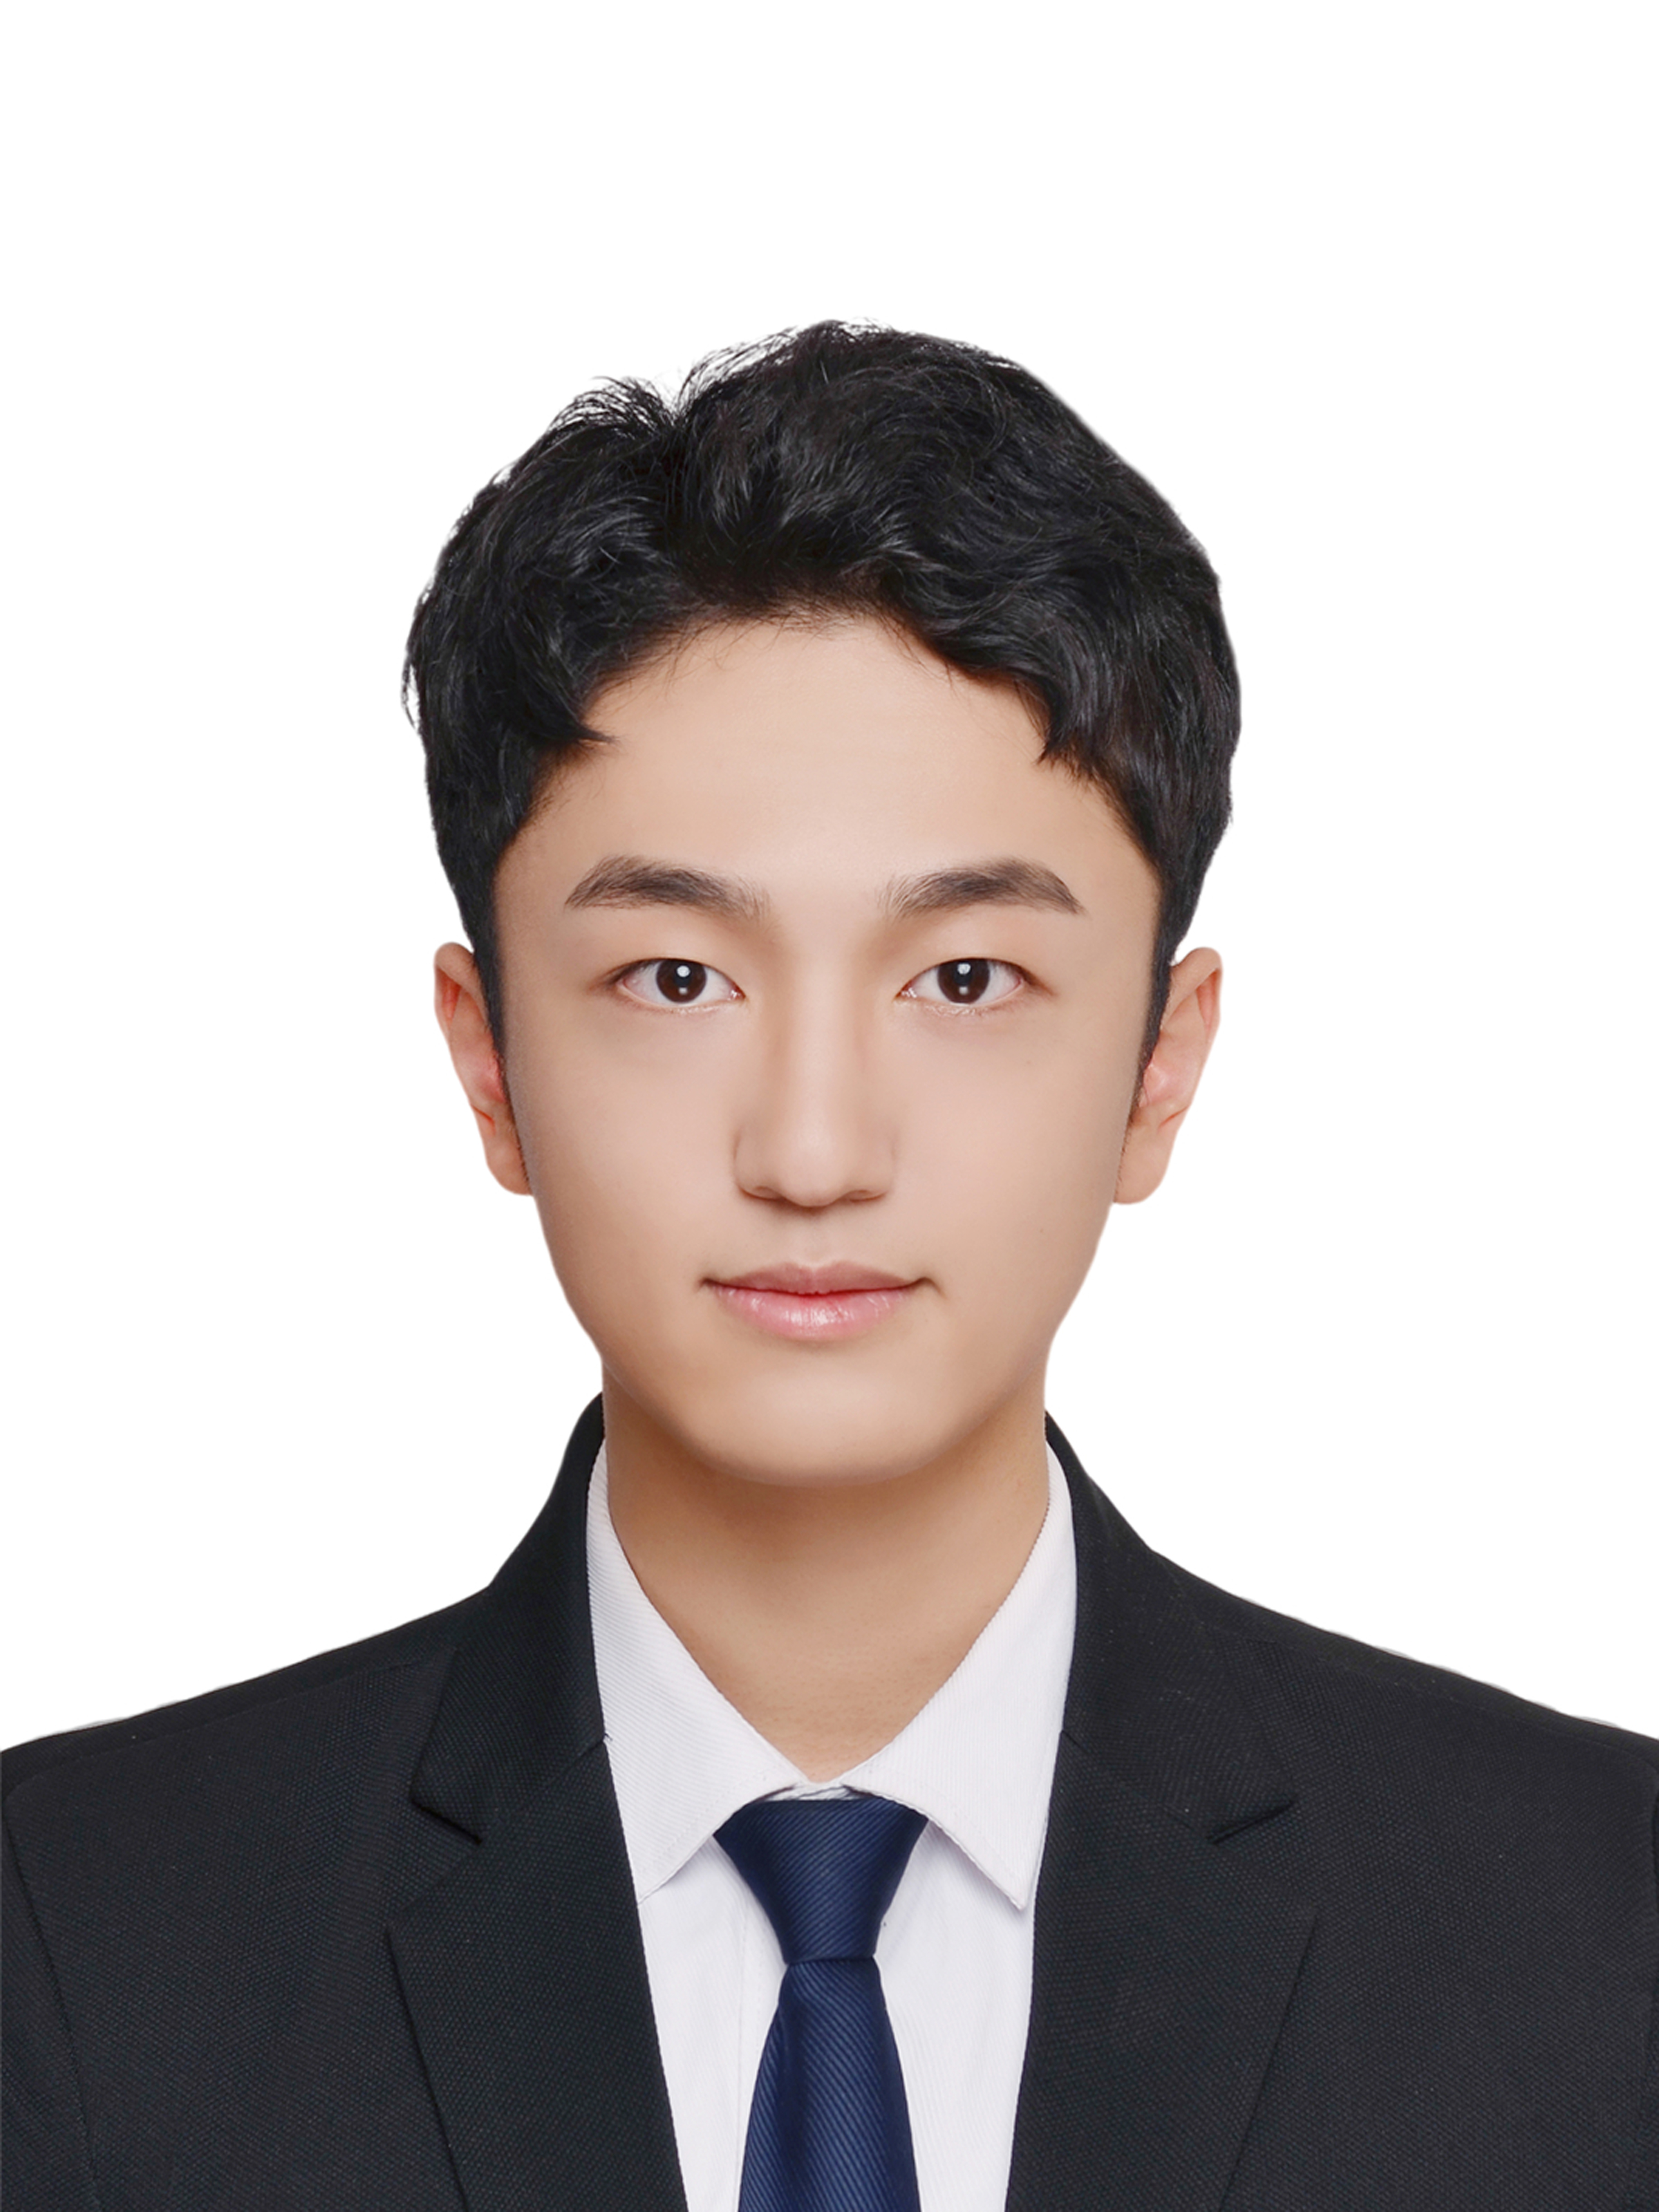
\includegraphics[width=1in,height=1.25in,clip,keepaspectratio]{fig/author/senwang.jpg}}]{Sen Wang} received the B.E. degree in Control Science and Engineering from Jilin University, Changchun, China, in 2023.
He is currently a third-year Ph.D. candidate in the Institute of Artificial Intelligence and Robotics at Xi’an Jiaotong University. His research interests include embodied computer vision, robotic manipulation and interactive world model. 
% He has published four papers in CVPR and NIPS.
\end{IEEEbiography}


\begin{IEEEbiography}[{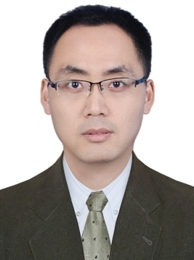
\includegraphics[width=1in,height=1.25in,clip,keepaspectratio]{fig/author/sanpingzhou.png}}]{Sanping Zhou} (Member, IEEE) received the Ph.D.
 degree in control science and engineering from Xi'an Jiaotong University, Xi’an, China, in 2020. From 2018 to 2019, he was a visiting Ph.D. student with
 Robotics Institute, Carnegie Mellon University. He is currently a professor with the Institute of Artificial Intelligence and Robotics, Xi'an Jiaotong University.
 His research interests include machine learning, deep learning, computer vision, and embodied AI, with a focus on person re-identification, salient object detection, medical image segmentation, image classification, and visual tracking.
\end{IEEEbiography}



% \begin{IEEEbiography}[{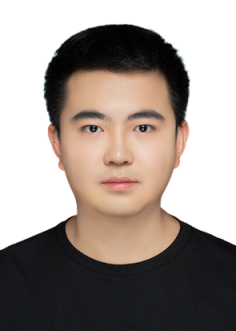
\includegraphics[width=1in,height=1.25in,clip,keepaspectratio]{fig/author/hch.png}}]{Hongcheng Huo} is an undergraduate student in Computer Science and Mathematics at the University of Toronto. His research experience includes work on multi-armed bandit algorithms in reinforcement learning, numerical analysis with a focus on high-performance computing and numerical optimization, and data-driven modeling using machine learning and deep learning. His academic interests focus on machine learning, deep learning, and efficient algorithmic modeling.
% \end{IEEEbiography}

\begin{IEEEbiography}[{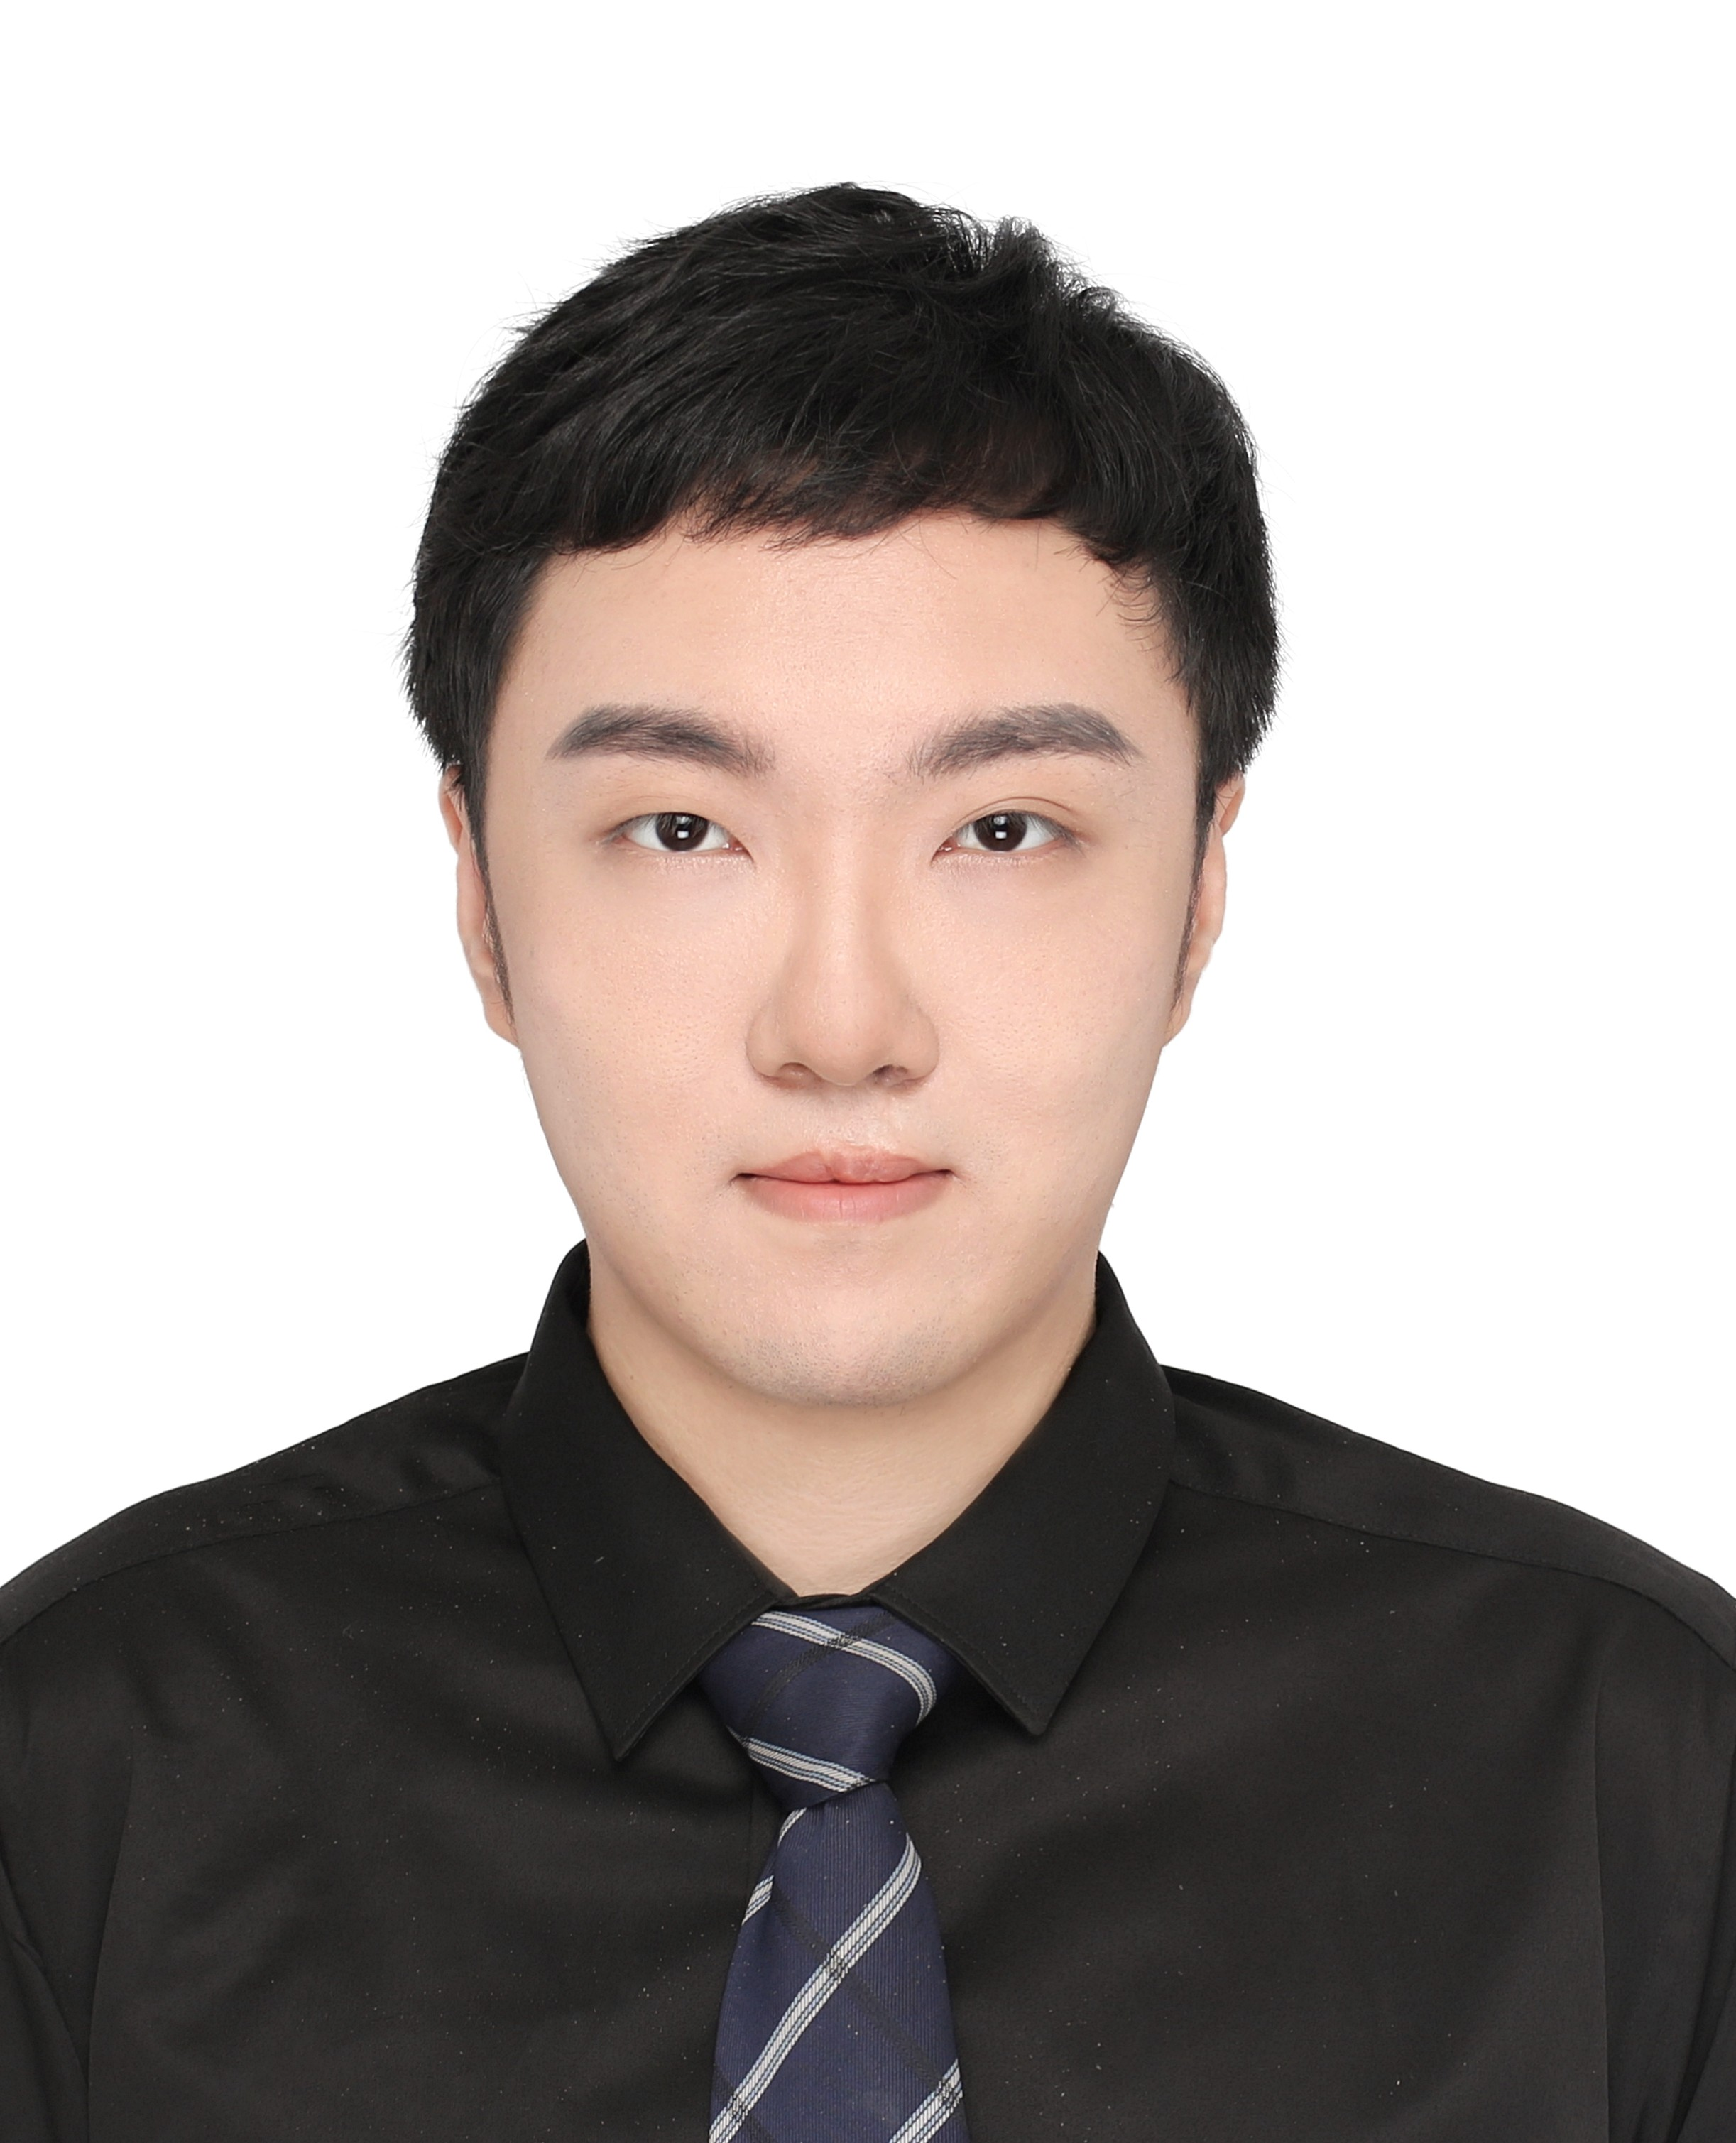
\includegraphics[width=1in,height=1.25in,clip,keepaspectratio]{fig/author/dhy.jpg}}]{Huaiyi Dong} received the B.E. degree in Software Engineering from China University of Geosciences,  wuhan, China, in 2023. He is currently a Ph.D. candidate in the Institute of Artificial Intelligence and Robotics at Xi’an Jiaotong University. His research interests include embodied computer vision and robotic manipulation. 
% He has published four papers in CVPR and NIPS.
\end{IEEEbiography}
\vspace{-6ex}

\begin{IEEEbiography}[{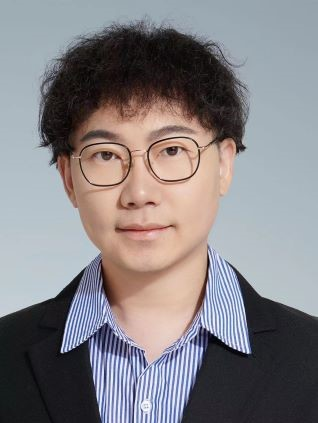
\includegraphics[width=1in,height=1.25in,clip,keepaspectratio]{fig/author/Kun-Xia.jpg}}]{Kun Xia} received the Ph.D. degree in Control Science and Engineering from Xi'an Jiaotong University, Xi'an, China, in 2024. From 2022 to 2023, he was a visiting Ph.D. student with University of Illinois Chicago, IL, USA. He is currently an Assistant Professor with the School of Computer Science and Technology, Xi'an Jiaotong University, Xi'an, China. His research interests include computer vision, image/video processing, analysis and understanding.
\end{IEEEbiography}
\vspace{-6ex}

\begin{IEEEbiography}[{\includegraphics[width=1in,height=1.25in,clip,keepaspectratio]{fig/author/Gang-Hua1.pdf}}]{Gang Hua}
(Fellow, IEEE) received the B.S. and M.S. degrees in automatic control engineering from Xi’an Jiaotong University, Xi’an, China, in 1999 and 2002, respectively, and the Ph.D. degree in electrical engineering and computer science from Northwestern University, Evanston, IL, USA, in 2006. He was a senior scientist with Microsoft Live labs Research from 2006 to 2009, a senior researcher with Nokia Research Center Hollywood from 2009 to 2010, a research staff member with IBM Research T. J. Watson Center from 2010 to 2011, and a visiting researcher from 2011 to 2014. During 2014–15, he took a leave and worked on the Amazon-Go project. He was an associate professor with the Stevens Institute of Technology from 2011 to 2015. He was also with Microsoft from 2015 to 2018 as the Science/Technical adviser to the CVP of the Computer Vision Group, director of Computer Vision Science Team in Redmond, Taipei ATL, and senior principal researcher/research manager with Microsoft Research. He was the CTO with Convenience Bee, and the managing director and chief scientist of its research branch in US, Wormpex AI Research, from 2018 to 2024. He was the vice president with Multimodal Experiences Research Lab, Dolby Laboratories from 2024 to 2025. He is currently the director of applied science with Amazon Alexa AI. His research interests include computer vision, pattern recognition, machine learning, robotics, towards general artificial intelligence, with primary applications in cloud and edge intelligence. He is an associate editor for TPAMI and MVA. He is a general chair of ICCV’2027 and a program chair of CVPR’2019 \& 2022. He is the recipient of the 2015 IAPR Young Biometrics Investigator Award. He is an IAPR Fellow and an ACM distinguished scientist.
\end{IEEEbiography}
\vspace{-6ex}

\begin{IEEEbiography}[{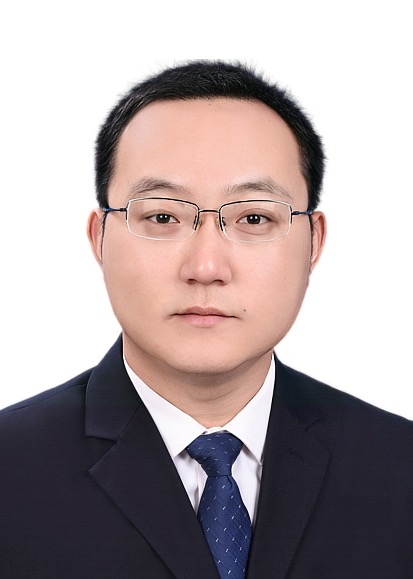
\includegraphics[width=1in,height=1.25in,clip,keepaspectratio]{fig/author/lewang.jpg}}]{Le Wang}(Senior Member, IEEE) received the B.S. and Ph.D. degrees in control science and engineering from Xi’an Jiaotong University, Xi’an, China, in 2008 and 2014, respectively. From 2013 to 2014, he was a visiting Ph.D. student with the Stevens Institute of Technology, Hoboken, NJ, USA. From 2016 to 2017, he was a visiting scholar with Northwestern University, Evanston, IL, USA. He is currently a professor with the Institute of Artificial Intelligence and Robotics, Xi’an Jiaotong University. His research interests include computer vision, pattern recognition, machine learning, and robotic manipulation. He is an associate editor for PR, MVA, and PRL.
\end{IEEEbiography}


